\documentclass[main.tex]{subfiles}

\begin{document}

In order to get a measurement of the Fierz term, a nucleus that beta decays is needed.
To put a limit on potential tensor terms, a Gamow-Teller transition is needed.
To do a proper percision shape measurement, a simple decay relatively close to stability is needed. 
In this measurement, the nucleus used was $^{20}$F.
 
\section{$^{20}$F Decay Characteristics}
The decay scheme is given in figure \ref{fig:DecayScheme}.

\begin{figure}[!htb]
	\centerline{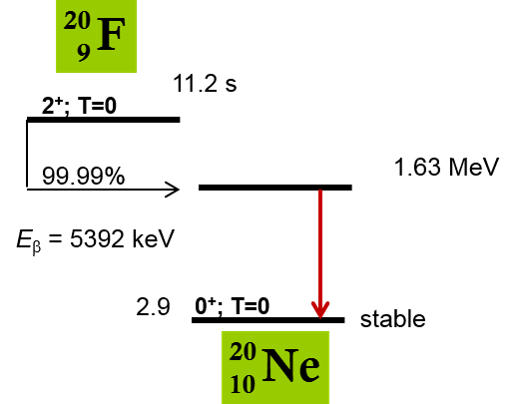
\includegraphics[width=0.78\textwidth]{20FDecayScheme.png}}
	\caption{The decay scheme of $^{20}$F.}
	\label{fig:DecayScheme}
\end{figure}

As seen in the figure, $^{20}$F decays 99.999\% of the time to the first excited state of $^{20}$Ne.
The $2^{+}$ state seen in the decay scheme is not the isobaric analogue state to the ground state of $^{20}$F.
That state is much higher in energy.
The beta decay therefor has a isospin change of 1, and is a Gamow-Teller transition.
The higher order matrix elements are very small.
This means the Fierz term is sensitive to potential tensor couplings.
The half-life of $^{20}$F is about 11 seconds. 
This is an important consideration for the experimental design.
The gamma ray and the end point energy of the electron are also important for the experimental design.
In order to get at the Fierz term, the beta decay spectrum shape must be described percisely.
The next chapter deals with the corrections to the beta decay spectrum.  

\section{Previous Measurments of $^{20}$F}

\end{document}
